\begin{center}
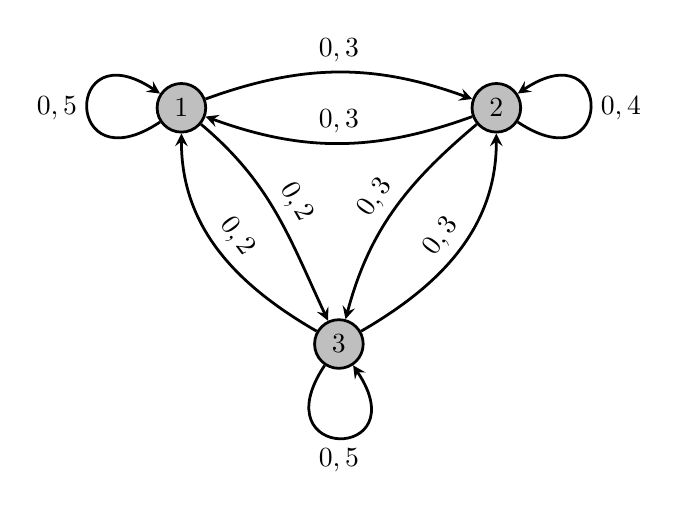
\begin{tikzpicture}[scale=1]
\tikzstyle{every path}=[>=stealth,->,line width=1pt];
\node [draw,circle,fill=gray!50] (A) at (0,0) {1};
\node [draw,circle,fill=gray!50] (B) at (4,0) {2};
\node [draw,circle,fill=gray!50] (C) at (2,-3) {3};
\draw[->] (A) to [out=20,in=160]  node[midway,sloped,above] {$0,3$}(B);
\draw[->] (A) to [out=-40,in=115]  node[midway,sloped,above] {$0,2$}(C);
\draw[->] (B) to [out=-160,in=-20] node[midway,sloped,above] {$0,3$} (A);
\draw[->] (B) to [out=-140,in=75] node[midway,sloped,above] {$0,3$} (C);
\draw[->] (C) to [out=150,in=-90] node[midway,sloped,above] {$0,2$} (A);
\draw[->] (C) to [out=30,in=-90] node[midway,sloped,above] {$0,3$} (B);
\draw[->] (B) .. controls +(1.5,-1) and +(1.5,1) .. node[midway,right]{$0,4$} (B) ;
\draw[->] (A) .. controls +(-1.5,-1) and +(-1.5,1) .. node[midway,left]{$0,5$} (A) ;
\draw[->] (C) .. controls +(-1,-1.5) and +(1,-1.5) .. node[midway,below]{$0,5$} (C) ;
\end{tikzpicture}
\end{center}